\documentclass[tikz,border=10pt]{standalone}
\usepackage{tikz}
\usepackage{amsmath,amssymb}
\usetikzlibrary{arrows.meta,calc,positioning,fit,backgrounds,decorations.pathreplacing}

\begin{document}
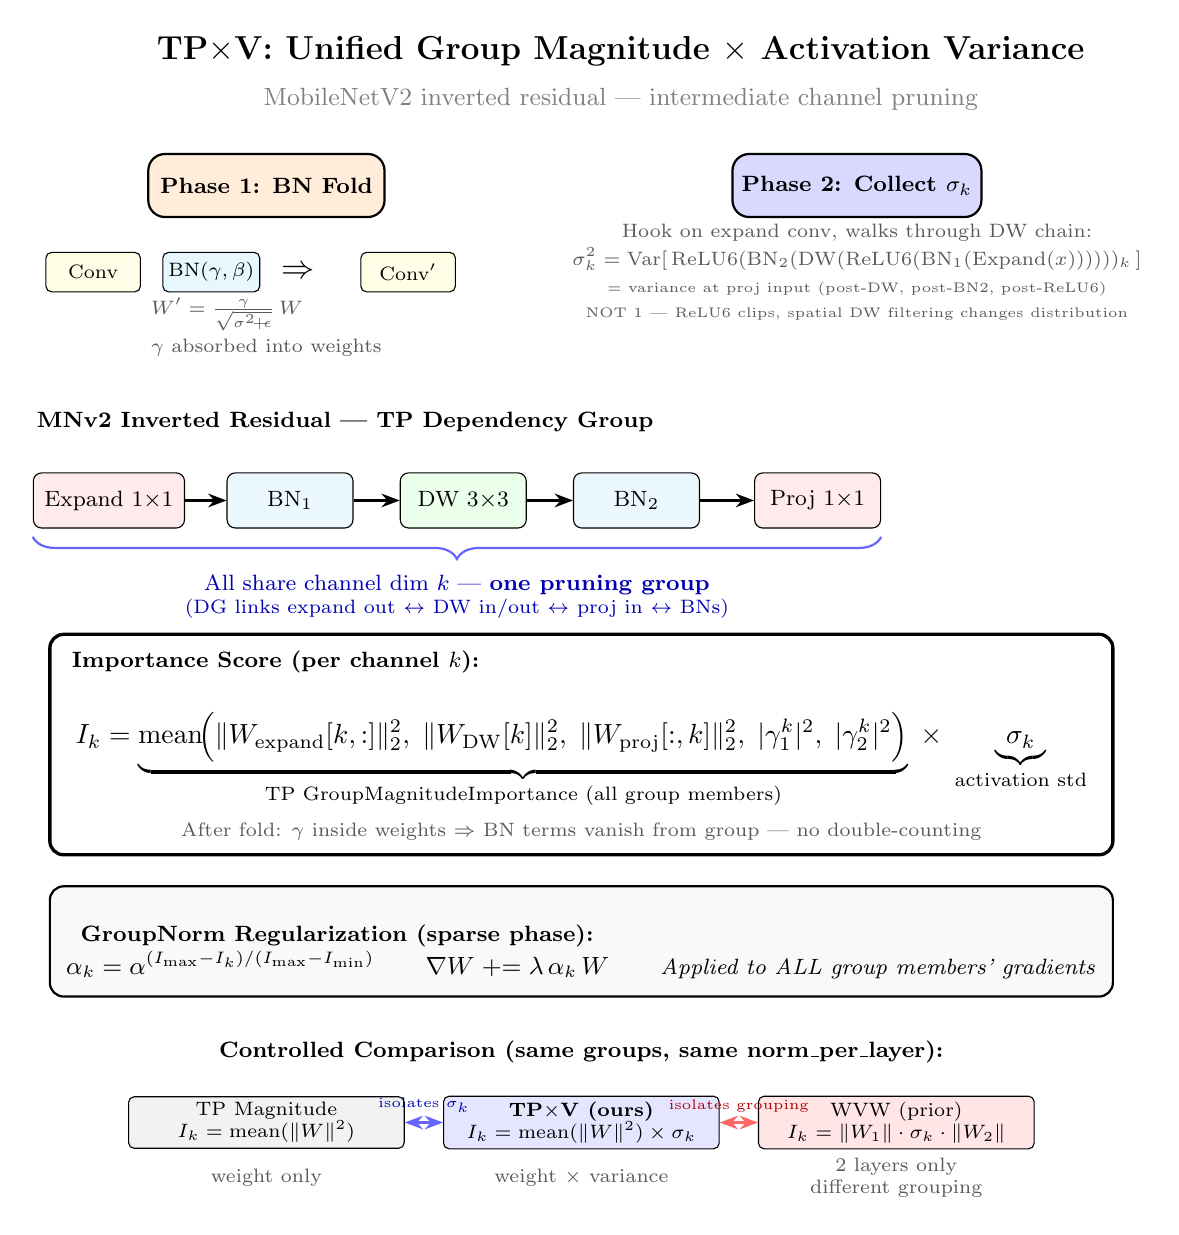
\begin{tikzpicture}[
  >=Stealth,
  box/.style={draw, rounded corners=3pt, minimum width=1.6cm, minimum height=0.7cm,
              inner sep=4pt, font=\footnotesize},
  smallbox/.style={draw, rounded corners=2pt, minimum width=1.2cm, minimum height=0.5cm,
              inner sep=2pt, font=\scriptsize},
  phase/.style={draw, rounded corners=6pt, thick, fill=#1, minimum width=3cm,
                minimum height=0.8cm, font=\footnotesize\bfseries},
  annot/.style={font=\scriptsize, text=gray!70!black},
  arr/.style={->, thick},
  dasharr/.style={->, thick, dashed, gray},
]

% ===== Title =====
\node[font=\large\bfseries] at (7, 11.5) {TP$\times$V: Unified Group Magnitude $\times$ Activation Variance};
\node[font=\small, text=gray] at (7, 10.9) {MobileNetV2 inverted residual --- intermediate channel pruning};

% ===== Phase 1: BN Fold =====
\node[phase=orange!15] (p1) at (2.5, 9.8) {Phase 1: BN Fold};

\node[smallbox, fill=yellow!10] (conv_pre) at (0.3, 8.7) {Conv};
\node[smallbox, fill=cyan!10] (bn_pre) at (1.8, 8.7) {BN($\gamma,\beta$)};
\node[font=\large] at (2.9, 8.7) {$\Rightarrow$};
\node[smallbox, fill=yellow!10] (conv_post) at (4.3, 8.7) {Conv$'$};
\node[annot, align=left] at (2.5, 8.0) {$W' = \frac{\gamma}{\sqrt{\sigma^2\!+\!\epsilon}}\,W$\\[2pt]
$\gamma$ absorbed into weights};

% ===== Phase 2: Collect Stats =====
\node[phase=blue!15] (p2) at (10, 9.8) {Phase 2: Collect $\sigma_k$};

\node[annot, align=center] at (10, 8.7) {Hook on expand conv, walks through DW chain:\\[2pt]
$\sigma_k^2 = \mathrm{Var}[\,\mathrm{ReLU6}(\mathrm{BN}_2(\mathrm{DW}(\mathrm{ReLU6}(\mathrm{BN}_1(\mathrm{Expand}(x))))))_k\,]$\\[2pt]
{\tiny = variance at proj input (post-DW, post-BN2, post-ReLU6)}\\[1pt]
{\tiny NOT 1 --- ReLU6 clips, spatial DW filtering changes distribution}};

% ===== MNv2 Block (group) =====
\node[font=\footnotesize\bfseries] at (3.5, 6.8) {MNv2 Inverted Residual --- TP Dependency Group};

% Block layers
\node[box, fill=red!8] (expand) at (0.5, 5.8) {Expand 1$\times$1};
\node[box, fill=cyan!8] (bn1) at (2.8, 5.8) {BN$_1$};
\node[box, fill=green!8] (dw) at (5.0, 5.8) {DW 3$\times$3};
\node[box, fill=cyan!8] (bn2) at (7.2, 5.8) {BN$_2$};
\node[box, fill=red!8] (proj) at (9.5, 5.8) {Proj 1$\times$1};

\draw[arr] (expand) -- (bn1);
\draw[arr] (bn1) -- (dw);
\draw[arr] (dw) -- (bn2);
\draw[arr] (bn2) -- (proj);

% Group brace
\draw[decorate, decoration={brace, amplitude=8pt, mirror}, thick, blue!60]
  ([yshift=-3pt]expand.south west) -- ([yshift=-3pt]proj.south east)
  node[midway, below=10pt, font=\footnotesize, blue!70!black, align=center]
  {All share channel dim $k$ --- \textbf{one pruning group}\\[-1pt]
   {\scriptsize (DG links expand out $\leftrightarrow$ DW in/out $\leftrightarrow$ proj in $\leftrightarrow$ BNs)}};

% ===== Criterion Box =====
\node[draw, rounded corners=5pt, very thick, fill=white, minimum width=13.5cm, minimum height=2.8cm,
      inner sep=8pt] (criterion) at (6.5, 2.7) {};
\node[font=\footnotesize\bfseries, anchor=north west] at ([xshift=5pt, yshift=-3pt]criterion.north west)
  {Importance Score (per channel $k$):};

\node[font=\normalsize, anchor=center] at (6.5, 2.5) {
  $I_k = \underbrace{\mathrm{mean}\!\Big(\|W_{\mathrm{expand}}[k,:]\|_2^2,\;
  \|W_{\mathrm{DW}}[k]\|_2^2,\;
  \|W_{\mathrm{proj}}[:,k]\|_2^2,\;
  |\gamma_1^k|^2,\;|\gamma_2^k|^2\Big)}_{\text{TP GroupMagnitudeImportance (all group members)}}
  \;\times\;
  \underbrace{\sigma_k}_{\text{activation std}}$
};

\node[annot, align=center] at (6.5, 1.6) {After fold: $\gamma$ inside weights $\Rightarrow$ BN terms vanish from group
--- no double-counting};

% ===== Regularization (below criterion) =====
\node[draw, rounded corners=5pt, thick, fill=gray!5, minimum width=13.5cm, minimum height=1.4cm,
      inner sep=6pt] (reg) at (6.5, 0.2) {};
\node[font=\footnotesize\bfseries, anchor=west] at ([xshift=8pt, yshift=2pt]reg.west)
  {GroupNorm Regularization (sparse phase):};
\node[font=\small, anchor=center] at (6.5, -0.1) {
  $\alpha_k = \alpha^{(I_{\max}-I_k)/(I_{\max}-I_{\min})}$\qquad
  $\nabla W \mathrel{+}= \lambda\,\alpha_k\,W$\qquad
  {\footnotesize\textit{Applied to ALL group members' gradients}}};

% ===== Comparison row =====
\node[font=\footnotesize\bfseries] at (6.5, -1.2) {Controlled Comparison (same groups, same norm\_per\_layer):};

\node[smallbox, fill=gray!10, minimum width=3.5cm, align=center] (tpmag) at (2.5, -2.1)
  {TP Magnitude\\$I_k = \mathrm{mean}(\|W\|^2)$};
\node[smallbox, fill=blue!10, minimum width=3.5cm, align=center] (tpv) at (6.5, -2.1)
  {\textbf{TP$\times$V (ours)}\\$I_k = \mathrm{mean}(\|W\|^2)\times\sigma_k$};
\node[smallbox, fill=red!10, minimum width=3.5cm, align=center] (wvw) at (10.5, -2.1)
  {WVW (prior)\\$I_k = \|W_1\|\cdot\sigma_k\cdot\|W_2\|$};

\node[annot] at (2.5, -2.8) {weight only};
\node[annot] at (6.5, -2.8) {weight $\times$ variance};
\node[annot, align=center] at (10.5, -2.8) {2 layers only\\different grouping};

% Arrow showing the isolation
\draw[<->, thick, blue!60] (tpmag.east) -- (tpv.west)
  node[midway, above, font=\tiny, blue!70!black] {isolates $\sigma_k$};
\draw[<->, thick, red!60] (tpv.east) -- (wvw.west)
  node[midway, above, font=\tiny, red!70!black] {isolates grouping};

\end{tikzpicture}
\end{document}
